\section{Merging datasets with siamese networks}
\label{joins}

Section~\ref{join_system} describes our overall system for using siamese networks for joins.  Section~\ref{join_complexity} provides a complexity analysis for this approach.


\section{Applying deep learning models to joins}
\label{join_system}
\begin{figure}
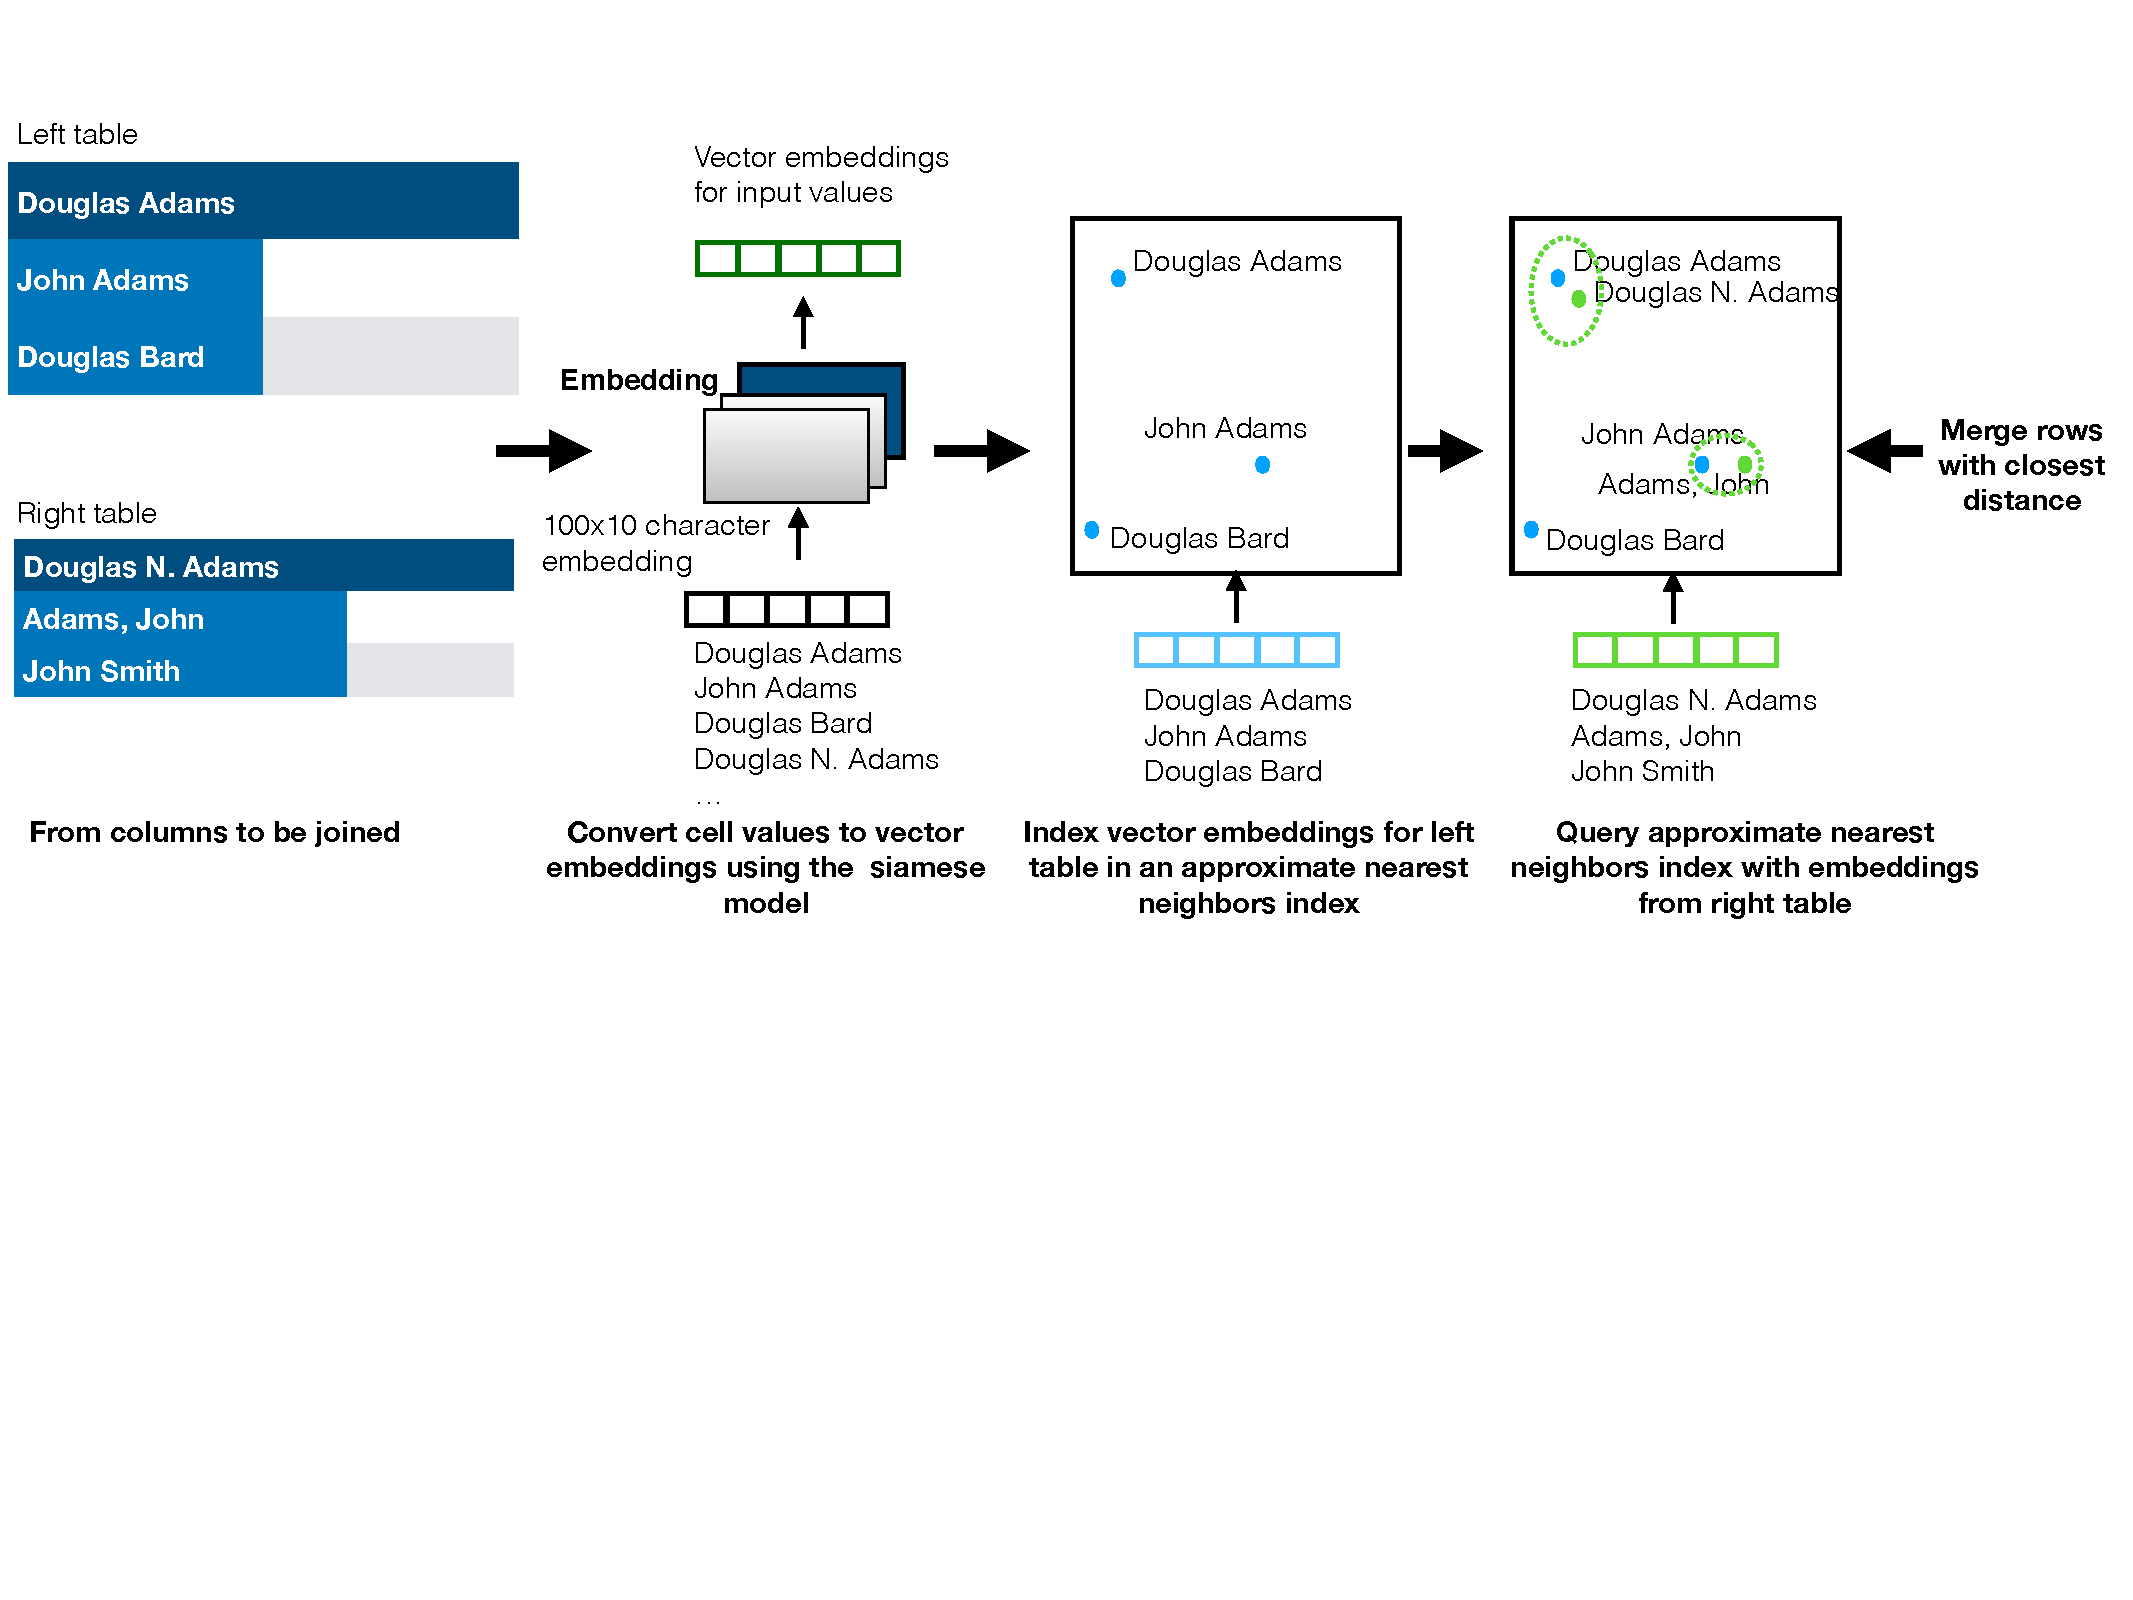
\includegraphics[width=1.0\linewidth]{joins}
\caption{Applying deep learning models to joins}
\label{join_fig}
\end{figure}

Figure~\ref{join_fig} provides an overview of how deep learning models can be used for merging datasets.  Panel (a) in the figure are the two datasets to be joined.  The datasets are labeled arbitrarily as a left table and a right table.  For each cell value in the two columns to be joined, we obtain vector embeddings from the siamese network that was used to estimate distance for same and different surface forms for the same entity.  Note that although the siamese network has three separate networks, each network within a triplet network is in fact identical to the other two networks because they share weights.  A single version of the network with learnt weights is used to generate the embeddings for the cell value as shown in panel (b). For the left table cell values, vector embeddings are inserted into an approximate nearest neighbors index, as shown in panel (c).  For each cell value in the right table, vector embeddings are used as `query vectors' to query the approximate nearest neighbors index as shown in panel (d).  In our context, merging the datasets would involve joining the top $k$ rows in the left table that are `closest' in distance to each cell value in the right table.  Note that the choice of $k$ clearly has a direct effect on the tradeoff between precision and recall, but this is true for any type of join algorithm that is not based on equality.


